% SICST manuscript - final academic version for C7
% Target journal: Requirements Engineering (Springer Nature)
% If the official Springer Nature class sn-jnl.cls is placed in this folder,
% this source can be migrated to that class for editorial submission.
\documentclass[10pt,a4paper]{article}

\usepackage[T1]{fontenc}
\usepackage[utf8]{inputenc}
\usepackage{lmodern}
\usepackage{microtype}
\usepackage[a4paper,margin=2.35cm]{geometry}
\usepackage{graphicx}
\usepackage{booktabs}
\usepackage{array}
\usepackage{tabularx}
\usepackage{longtable}
\usepackage{enumitem}
\usepackage{natbib}
\usepackage{hyperref}
\usepackage{url}
\usepackage{caption}
\usepackage{float}
\usepackage{setspace}
\usepackage{xcolor}
\usepackage{amsmath}
\usepackage{amssymb}
\usepackage{titlesec}

\hypersetup{colorlinks=true,linkcolor=black,citecolor=black,urlcolor=black}
\setstretch{1.04}
\setlength{\parindent}{1.2em}
\setlength{\parskip}{0.25em}
\titleformat{\section}{\large\bfseries}{\thesection}{0.6em}{}
\titleformat{\subsection}{\normalsize\bfseries}{\thesubsection}{0.6em}{}
\captionsetup{font=small,labelfont=bf}

\title{\textbf{Evidence-Driven Requirements Engineering for an Intelligent Physical Therapy Follow-Up System: The SICST Case Study}}

\author{Kevin Germán Contreras Chávez \and Angelo Paul Zambrano Moya\\
\small Universidad Técnica Estatal de Quevedo (UTEQ), Ecuador\\
\small Software Engineering Program -- Requirements Engineering (ISR-401)\\
\small Corresponding author: Angelo Paul Zambrano Moya\\
\small ORCID: 0009-0006-0056-8482}

\date{Manuscript version 1.0 -- September 2026\\
\small Target journal: \textit{Requirements Engineering} (Springer Nature)}

\begin{document}
\maketitle

\begin{abstract}
Digital support for home-based physical therapy must translate heterogeneous stakeholder needs into requirements that are clinically cautious, understandable, privacy-aware, and technically verifiable. This paper reports an evidence-driven requirements engineering case study for SICST, an intelligent system for control and follow-up of physical therapy. The study consolidated a questionnaire with 79 coded responses (62 patients or former patients, 14 relatives or caregivers, and 3 physiotherapists), an interview corpus of 11 patient sessions for thematic analysis, walkthrough evidence, traceability artifacts, and two role-specific web prototypes. Qualitative analysis used a 12-code book and a binary evidence matrix. The corpus reached 12 accumulated subthemes by the eighth interview and added no new subthemes in the final three interviews. A second independent coding covered 3 of the 11 interviews (27.27\% of the corpus), with 36 comparable decisions, 91.67\% agreement, Cohen's $\kappa=0.7187$, and a bootstrap 95\% confidence interval of [0.3077, 1.0000]. The most recurrent needs concerned execution supervision, adherence and reminders, dosing instructions, pain/fatigue recording, progress follow-up, privacy, and authorized access. These findings were propagated into a traceability baseline containing 58 documented requirement traces: 33 functional requirements, 15 general non-functional requirements, and 10 AI-specific non-functional requirements. The resulting MVP separates patient and physiotherapist workflows and makes privacy, consent, progress monitoring, alerts, and human supervision explicit. The study demonstrates how field evidence, qualitative saturation, inter-coder agreement, and end-to-end traceability can be combined in a small applied requirements engineering project without presenting synthetic evaluation data as participant evidence.
\end{abstract}

\noindent\textbf{Keywords:} requirements engineering; physical therapy; rehabilitation; intelligent systems; traceability; explainability; privacy; qualitative coding; reproducibility; human oversight.

\section{Introduction}
Physical therapy frequently extends beyond the clinical session. Patients may be expected to remember exercises, execute movements correctly, respect repetition and rest instructions, report pain or fatigue, and communicate problems between appointments. These activities create a requirements problem before they create an algorithmic problem: a digital system must first represent the needs, constraints, responsibilities, and safety expectations of patients, caregivers, and professionals in a way that can be verified and traced.

Requirements engineering (RE) provides the methods needed to elicit, analyze, document, validate, prioritize, and manage such expectations \citep{pohl2010requirements,iso29148_2018,sommerville2016software}. In health-related software, however, functional completeness is not sufficient. Privacy, usability, data protection, explainability, human oversight, and clinical safety must be treated as explicit system qualities rather than informal intentions \citep{iso25010_2023,chung2009nfr,chazette2020explainability}. These concerns are especially relevant when a proposed system includes camera-based analysis or intelligent assistance, because automated outputs must remain understandable and subordinate to professional judgment.

SICST (\textit{Sistema Inteligente de Control y Seguimiento de Terapia Física}) was developed as an academic case study in Requirements Engineering at Universidad Técnica Estatal de Quevedo. The project addresses follow-up of physical therapy routines by separating patient and physiotherapist interactions while maintaining a common traceability chain from field evidence to requirements, design elements, prototype behavior, and conceptual tests.

The project originally accumulated heterogeneous artifacts: interviews, walkthroughs, questionnaires, consent records, UML models, requirement matrices, prototype demonstrations, and an experimental protocol. The principal methodological challenge was therefore not merely to produce more documentation, but to consolidate this evidence into a reproducible argument: what needs appeared in the field, how consistently they appeared, how they were transformed into requirements, and whether the resulting requirements remained traceable through design and validation artifacts.

This paper reports that consolidation. It deliberately excludes synthetic experimental rounds from participant-based empirical claims. The repository explicitly labels those rounds as a controlled simulation, so they are not treated here as clinical, usability, or human-subject results. Instead, the paper focuses on the real questionnaire and qualitative evidence, the coded thematic structure, the traceability baseline, and the resulting MVP.

The study addresses three research questions:

\begin{description}[leftmargin=1.3cm,labelwidth=1.0cm]
\item[RQ1.] Which recurrent needs and concerns emerge from the field evidence for home-based physical therapy follow-up?
\item[RQ2.] How can these needs be transformed into a verifiable requirements baseline that includes privacy, safety, explainability, and human oversight?
\item[RQ3.] To what extent is the resulting evidence-to-requirement chain auditable through thematic saturation, inter-coder agreement, traceability, and reproducible data artifacts?
\end{description}

The contribution is a documented RE case study rather than a claim of clinical effectiveness. Its value lies in showing how a small academic team can connect field evidence to a requirements baseline while explicitly representing uncertainty, limitations, and reproducibility.

\section{Background and Related Work}
\subsection{Requirements engineering in evidence-rich domains}
RE is concerned with discovering and negotiating stakeholder goals, documenting system behavior and constraints, and maintaining coherence as the solution evolves \citep{pohl2010requirements,iso29148_2018}. Traceability is central because it allows a requirement to be connected backward to its source and forward to design and verification artifacts. This relationship is particularly useful when requirements are derived from mixed evidence such as interviews, questionnaires, observations, and validation sessions.

Applied software engineering studies benefit from transparent case-study procedures, explicit data sources, and clear chains of evidence \citep{runeson2009guidelines}. In SICST, this principle was implemented as a documentary chain linking source evidence to functional or non-functional requirements, use cases, conceptual classes, states, BDD-style scenarios, and conceptual test cases.

\subsection{Physical therapy follow-up and telerehabilitation}
Telerehabilitation and technology-supported rehabilitation have been studied as mechanisms for extending therapeutic support beyond face-to-face sessions \citep{munoztomas2023telerehabilitation,susomarti2021effectiveness,gava2022shoulder}. The literature reports potential benefits of remote access and exercise support, while also emphasizing the need for appropriate intervention design and professional supervision. Computer vision approaches can assist with posture or movement analysis \citep{debnath2022rehabilitation,cao2021openpose,lugaresi2019mediapipe}, but the presence of a technical capability does not by itself justify its use. The decision to use camera-derived information must be grounded in requirements concerning consent, purpose, data minimization, interpretability, and override mechanisms.

\subsection{Explainability and non-functional requirements}
Explainability can be treated as a non-functional requirement when the system must communicate why an automated result or recommendation was produced \citep{chazette2020explainability}. General explainable-AI methods such as local surrogate explanations or feature attribution have been proposed in machine learning \citep{ribeiro2016lime,lundberg2017shap}, while health contexts require an additional layer of caution because the user may interpret an explanation as clinical advice \citep{holzinger2017xai}. Therefore, SICST specifies explainability together with human supervision rather than as a replacement for professional decision-making.

\subsection{Qualitative saturation and agreement}
Qualitative coding requires a defensible account of how themes were identified and when additional material stopped producing new categories. Distinctions between code saturation and meaning saturation are well established \citep{hennink2017codesaturation}, and interview counts should be interpreted in relation to the scope and homogeneity of the study rather than as universal thresholds \citep{guest2006interviews}. In addition, when more than one person codes the same material, reporting agreement with an uncertainty interval provides stronger evidence than a single percentage alone.

\section{Case Study Design}
\subsection{Context and scope}
SICST was developed in 2026 within the Software Engineering program at UTEQ as a requirements engineering project focused on intelligent follow-up of physical therapy. The intended system is not a medical device claim and the academic prototype is not presented as a substitute for diagnosis, prescription, or professional supervision. The target workflows cover patient follow-up and physiotherapist management, including routines, exercise guidance, pain and fatigue reporting, progress, alerts, privacy, and consent.

The study uses an evidence-driven case-study design \citep{runeson2009guidelines}. The unit of analysis is the requirements baseline of SICST and the principal question is how field evidence is translated into requirements and traceability artifacts.

\subsection{Data sources}
The current reproducible dataset contains 79 coded questionnaire responses. The profile distribution is shown in Fig.~\ref{fig:profiles}: 62 responses correspond to patients or former physical-therapy patients, 14 to relatives or caregivers, and 3 to physiotherapists. The questionnaire includes closed questions concerning exercise adherence, clarity of instructions, reminders, pain and fatigue, progress visualization, camera use, privacy, and access, as well as professional questions for physiotherapists.

\begin{figure}[H]
\centering
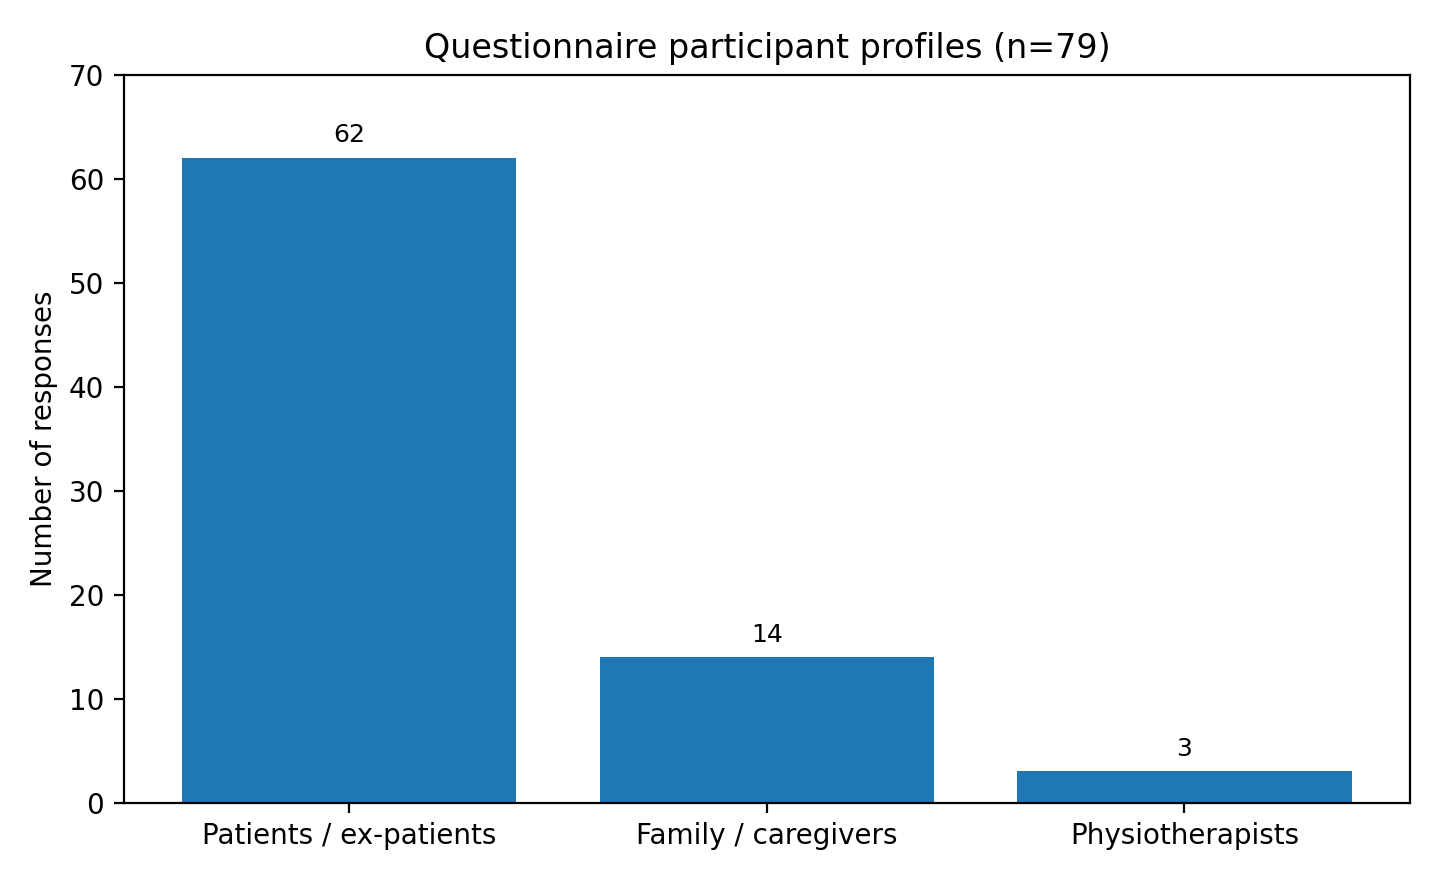
\includegraphics[width=0.86\textwidth]{figuras/figura_perfiles.png}
\caption{Profile distribution of the reproducible questionnaire dataset ($n=79$).}
\label{fig:profiles}
\end{figure}

The principal qualitative corpus contains 11 patient interviews. Walkthrough sessions are maintained as complementary triangulation evidence but are not artificially counted as additional interviews. A 12-subtheme codebook was used to classify evidence by presence (1) or absence (0) in each interview. The codes are listed in Table~\ref{tab:codes}.

\begin{table}[H]
\centering
\small
\caption{Thematic codebook used in the qualitative analysis.}
\label{tab:codes}
\begin{tabularx}{\textwidth}{>{\bfseries}p{1.4cm}p{3.2cm}X}
\toprule
Code & Parent category & Subtheme \\
\midrule
SUB-01 & Adherence & Adherence and reminders \\
SUB-02 & Understanding & Instructions and dosage \\
SUB-03 & Understanding & Audiovisual support \\
SUB-04 & Correction & Supervision and execution correction \\
SUB-05 & Clinical safety & Pain and fatigue recording \\
SUB-06 & Follow-up & Progress follow-up \\
SUB-07 & Follow-up & Communication with physiotherapist \\
SUB-08 & Privacy & Camera and data privacy \\
SUB-09 & Privacy & Authorized family access \\
SUB-10 & Clinical safety & Safety and warning signs \\
SUB-11 & Understanding & Accessibility and ease of use \\
SUB-12 & Follow-up & Centralized organization \\
\bottomrule
\end{tabularx}
\end{table}

\subsection{Qualitative analysis procedure}
Each of the 11 interviews was compared with the operational definitions in the codebook. A code was assigned only when sufficient evidence supported the subtheme. A zero indicates absence of sufficient evidence in that interview; it does not indicate participant disagreement.

The sequence of first appearances was recorded in a saturation table. The cumulative number of subthemes was then plotted against interview order. A second independent coding was performed on 3 of the 11 interviews, representing 27.27\% of the corpus. Agreement was calculated over the binary coding decisions before reconciliation. Cohen's kappa and a bootstrap confidence interval were produced by a versioned script using 10,000 resamples and seed 401.

\subsection{Questionnaire processing and reproducibility}
The reproducible data package is stored under \texttt{07\_Datos/}. The raw CSV is processed only through a versioned Python orchestrator. The processing step removes the timestamp from the derived dataset, trims leading and trailing whitespace, discards only fully empty rows, preserves participant responses, generates the profile summary, and writes SHA-256 checksums. No participants or responses are generated by the script.

The one-command entry point documented by the project is:

\begin{quote}
\texttt{python 07\_Datos/scripts/orquestar.py}
\end{quote}

The package includes raw and processed data, results, a data dictionary, data-use conditions, checksums, a deviations file, and a persistent-deposit record.

\subsection{Requirements consolidation and traceability}
Field evidence was transformed into functional and non-functional requirements according to standard RE practices \citep{iso29148_2018,pohl2010requirements}. Non-functional requirements were treated as measurable constraints rather than general aspirations, particularly for privacy, usability, explainability, equity, monitoring, and human supervision.

The current traceability baseline contains 58 documentary traces: 33 functional requirements, 15 general non-functional requirements, and 10 AI-specific non-functional requirements. The main traceability chain is:

\begin{center}
\textbf{Source $\rightarrow$ RF/RNF $\rightarrow$ Use Case $\rightarrow$ UML Class $\rightarrow$ State $\rightarrow$ BDD $\rightarrow$ Test Case}
\end{center}

All 58 traces are documented as complete in the repository baseline. For the 33 functional requirements, the backlog-to-specification synchronization is 33/33.

\subsection{Prototype as validation support}
The MVP is separated into two independent web applications: one for physiotherapists and one for patients. The physiotherapist application represents patient management, initial assessment, exercise catalogues, routine assignment, therapeutic follow-up, alerts, reports, privacy, and consent. The patient application represents routine consultation, guided exercises, pain and fatigue registration, progress tracking, reminders, privacy, and camera consent. The prototype is used as validation support for the requirements; it is not treated as evidence of clinical effectiveness.

\section{Results}
\subsection{RQ1: recurrent needs from field evidence}
Table~\ref{tab:freq} summarizes the presence of the 12 coded subthemes across the 11 interview corpus. Supervision and execution correction (SUB-04) appeared in all 11 interviews. Adherence and reminders (SUB-01), instructions and dosage (SUB-02), pain/fatigue recording (SUB-05), and progress follow-up (SUB-06) each appeared in 10 of 11 interviews (90.9\%). Privacy of camera and data (SUB-08) appeared in 8 interviews (72.7\%), and authorized family access (SUB-09) appeared in 7 (63.6\%). Audiovisual support and warning signs each appeared in 5 interviews (45.5\%). Communication with the physiotherapist appeared in 4 (36.4\%). Accessibility/ease of use and centralized organization were less frequent in the binary matrix but remained explicit requirements because low frequency does not imply low importance in safety- or accessibility-related contexts.

\begin{table}[H]
\centering
\small
\caption{Frequency of coded subthemes in the 11-interview corpus.}
\label{tab:freq}
\begin{tabular}{lrr}
\toprule
Code & Interviews & Percentage \\
\midrule
SUB-01 & 10 & 90.9\% \\
SUB-02 & 10 & 90.9\% \\
SUB-03 & 5 & 45.5\% \\
SUB-04 & 11 & 100.0\% \\
SUB-05 & 10 & 90.9\% \\
SUB-06 & 10 & 90.9\% \\
SUB-07 & 4 & 36.4\% \\
SUB-08 & 8 & 72.7\% \\
SUB-09 & 7 & 63.6\% \\
SUB-10 & 5 & 45.5\% \\
SUB-11 & 1 & 9.1\% \\
SUB-12 & 2 & 18.2\% \\
\bottomrule
\end{tabular}
\end{table}

\begin{figure}[H]
\centering
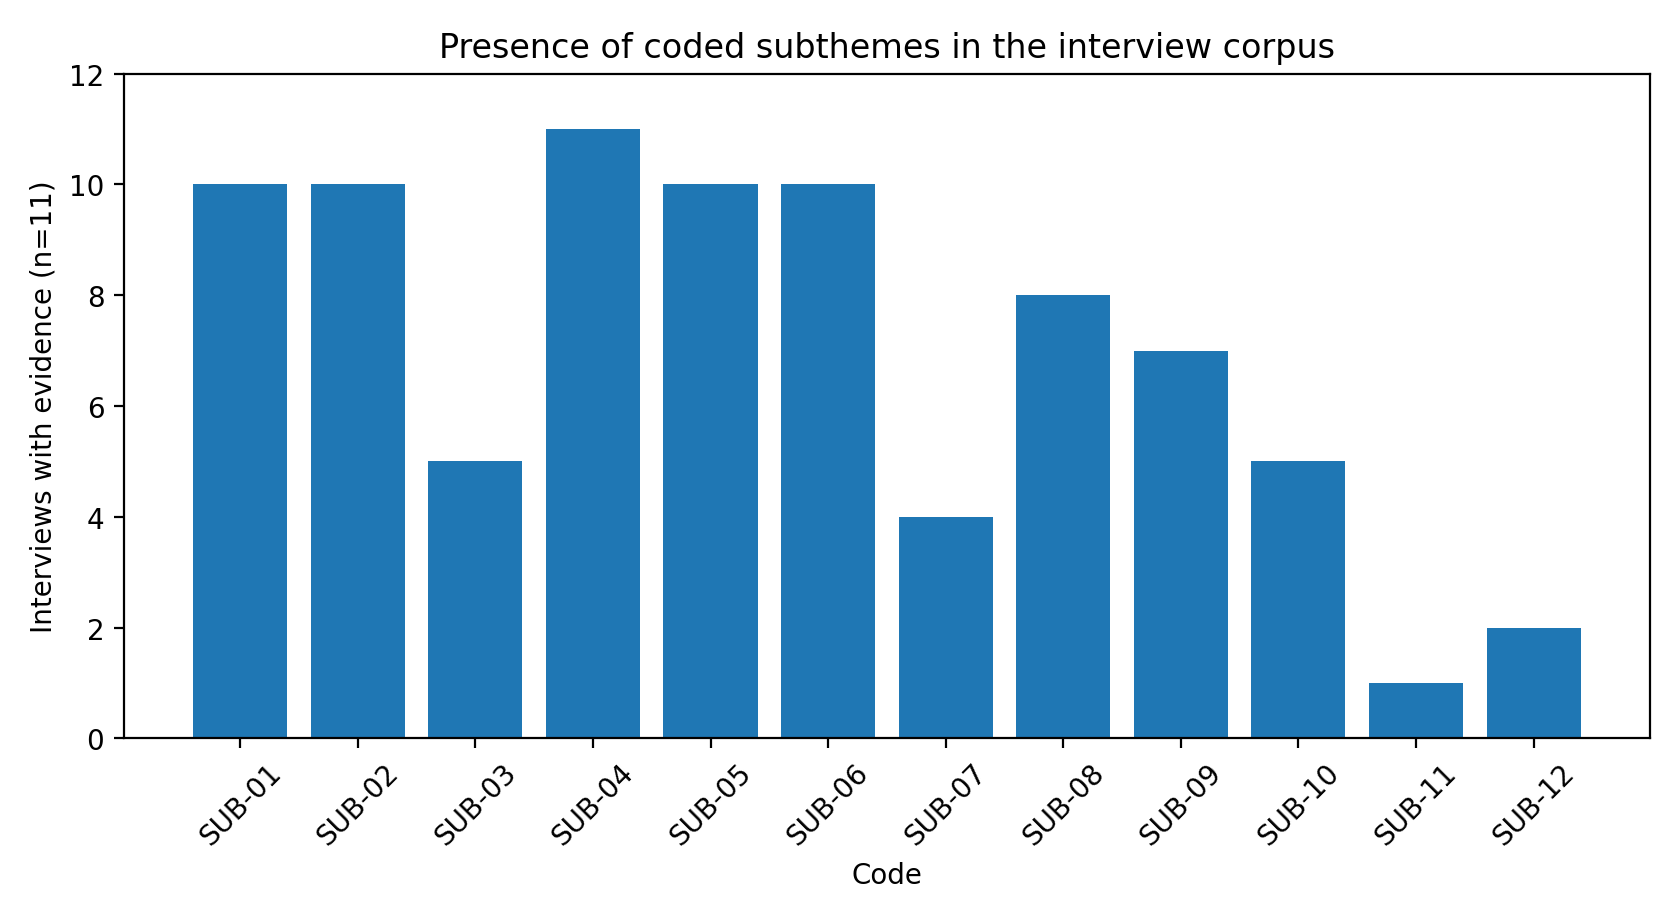
\includegraphics[width=0.88\textwidth]{figuras/figura_subtemas.png}
\caption{Presence of the 12 coded subthemes across the interview corpus.}
\label{fig:subthemes}
\end{figure}

The pattern supports a requirements interpretation centered on five clusters: (1) adherence and understandable dosing, (2) execution correction, (3) symptom and progress monitoring, (4) privacy and authorized access, and (5) safety and professional communication. These clusters are consistent with the questionnaire domains and the two user-role workflows implemented in the MVP.

\subsection{Saturation}
The first interview introduced 8 of the 12 subthemes. Interviews 2, 4, 6, and 8 each added one new subtheme; interviews 3, 5, and 7 added none. The corpus reached all 12 observed subthemes by interview 8, after which interviews 9, 10, and 11 added no new subthemes (Fig.~\ref{fig:saturation}). This pattern is evidence of code saturation within the bounded scope of the current codebook, not proof that every possible meaning in the broader population has been exhausted \citep{hennink2017codesaturation}.

\begin{figure}[H]
\centering
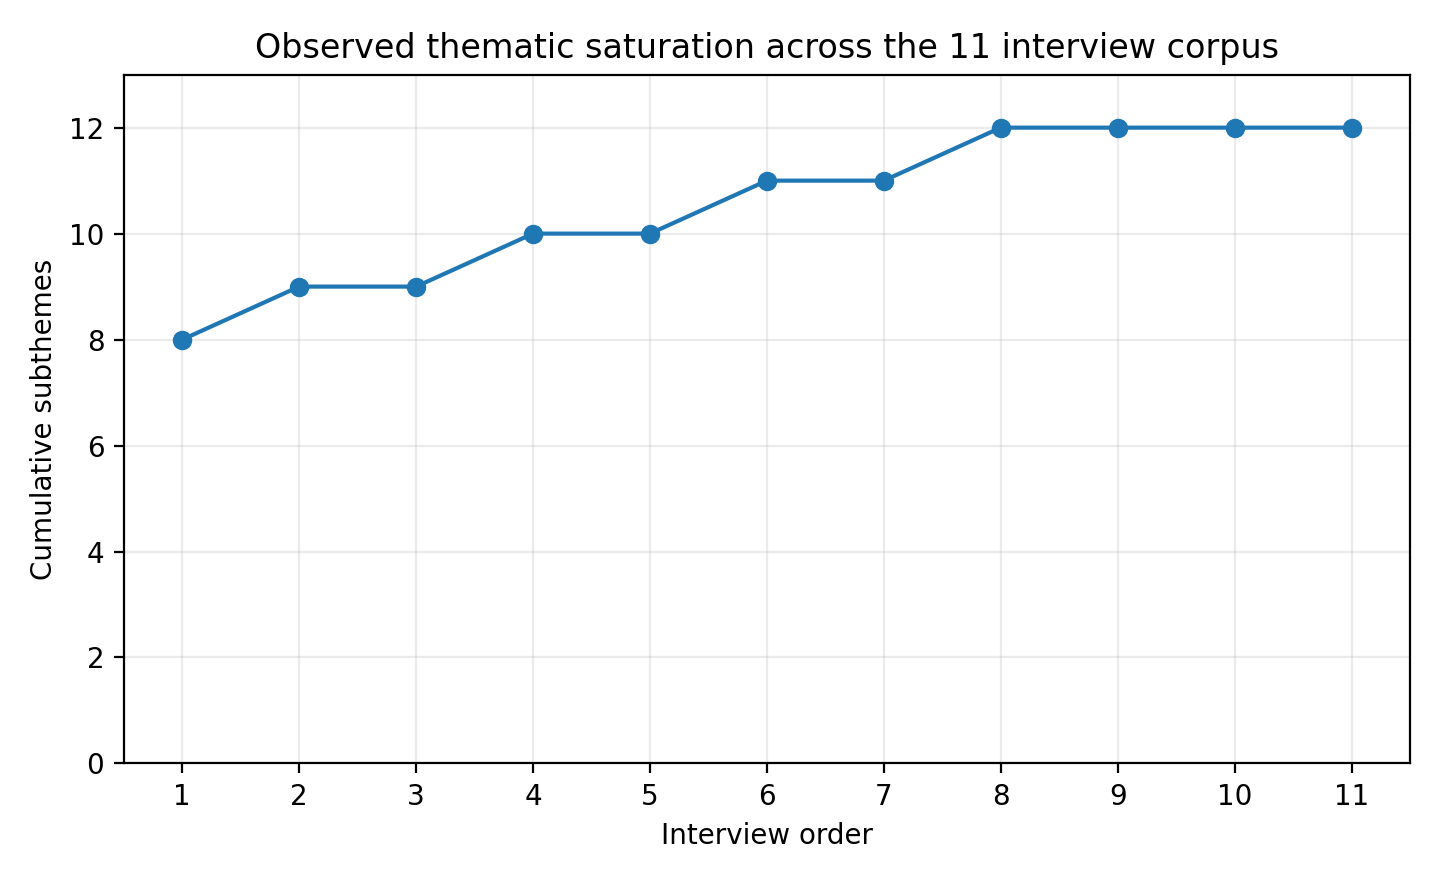
\includegraphics[width=0.86\textwidth]{figuras/figura_saturacion.png}
\caption{Cumulative subthemes across the 11-interview sequence. The final three interviews added no new subthemes.}
\label{fig:saturation}
\end{figure}

\subsection{Independent double coding}
The independent second coding covered 3 of the 11 interviews (27.27\%). Across 36 coding decisions, the two coders agreed on 33 and disagreed on 3, yielding 91.67\% observed agreement. Cohen's kappa was 0.7187. The bootstrap 95\% confidence interval was [0.3077, 1.0000]. The wide interval reflects the limited amount of double-coded material and should be interpreted as uncertainty around a promising point estimate rather than as proof of near-perfect reliability.

The agreement analysis was performed before reconciliation. This preserves the independence of the comparison and avoids inflating the reported agreement by resolving disagreements first.

\subsection{RQ2: translation into a verifiable requirements baseline}
The field evidence was transformed into a baseline that distinguishes functional behavior from non-functional constraints. The 33 functional requirements cover core workflows such as patient management, therapeutic routines, exercise consultation, symptom registration, progress review, alerts, and reporting. The 15 general non-functional requirements cover qualities such as usability, privacy, integrity, and performance. Ten additional AI-specific non-functional requirements document constraints for the intelligent component.

The thematic evidence explains why several requirements are central. SUB-04 supports execution-feedback and supervision requirements; SUB-05 and SUB-10 support symptom logging, alerting, and safety constraints; SUB-08 and SUB-09 support consent, access control, and privacy requirements; SUB-01 and SUB-02 support reminders and clear dosing; SUB-06 supports progress visualization and therapist follow-up.

For the intelligent component, the requirements baseline makes human authority explicit. Automated assistance is framed as support: the physiotherapist must remain able to review or override an indication, and the system must record relevant decisions. This design principle is consistent with the need to avoid turning an explainability mechanism into an apparent clinical authority \citep{chazette2020explainability,holzinger2017xai}.

\subsection{RQ3: auditability and reproducibility}
Auditability is supported by four complementary mechanisms. First, the qualitative corpus has a codebook, binary matrix, saturation table, and generated saturation figure. Second, independent double coding is reported with both kappa and an uncertainty interval. Third, the requirements baseline has 58 complete documentary traces that connect sources to downstream artifacts. Fourth, the questionnaire package can be regenerated by a single script and verified using SHA-256 checksums.

The dataset version used by this manuscript was deposited in Zenodo as version 1.0 with DOI \href{https://doi.org/10.5281/zenodo.22315298}{10.5281/zenodo.22315298}. The deposit contains reproducibility materials and metadata, while direct identifiers and signed consent documents are excluded from the public data package.

\section{Discussion}
\subsection{From recurrent needs to system structure}
The results show that the strongest recurring concerns are not exotic AI functions. They are practical requirements: correct execution, clear instructions, adherence, pain and fatigue recording, and visible progress. This is an important design signal. In an intelligent rehabilitation system, the value of automation depends on whether basic workflow and communication needs are already represented correctly.

The 100\% presence of supervision/correction in the interview matrix is particularly relevant. It supports the decision to represent movement feedback and therapist oversight as first-class capabilities. However, the requirement should not be interpreted as evidence that an automated camera module is clinically validated. The field evidence establishes a user need for correction; it does not validate a particular computer-vision algorithm.

Similarly, privacy appeared frequently and was reinforced by questionnaire items concerning camera authorization and access. This supports a consent-driven architecture in which camera use is optional and purpose-bound. The Ecuadorian data-protection context further motivates data minimization, restricted access, and separation of public derived data from restricted identifiable evidence \citep{ecuador2021lopdp}.

\subsection{Why traceability matters in this case}
The traceability baseline is one of the strongest outcomes of the project. A field code such as SUB-05 is not useful by itself unless it can be connected to a requirement that states what the system must do, a design element that realizes it, and a test condition that can verify it. The 58-trace baseline operationalizes that chain and reduces the risk that field findings remain isolated from implementation decisions.

This is also relevant for change management. If a privacy or safety finding changes, the traceability chain identifies which use cases, classes, states, scenarios, and tests must be revisited. Such bidirectional reasoning is a core advantage of disciplined RE \citep{pohl2010requirements,iso29148_2018}.

\subsection{Interpreting the agreement result}
A kappa of 0.7187 indicates substantial consistency in the current coding exercise, but the confidence interval is broad. The point estimate therefore supports the plausibility of the codebook while the interval prevents overconfidence. The result is stronger than reporting only a percentage agreement because it accounts for chance agreement, yet it remains limited by the small number of double-coded interviews and binary decisions.

The double-coding proportion (27.27\%) exceeds the project's required minimum of 20\% of the corpus. More extensive double coding would narrow uncertainty and permit sensitivity analyses by code category. The present result should therefore be seen as an auditable quality-control step rather than a definitive reliability study.

\subsection{Relationship between questionnaire and interviews}
The questionnaire and interviews serve different roles. The questionnaire broadens coverage across 79 coded responses and three stakeholder profiles, while interviews provide richer evidence for recurring needs and saturation. The manuscript does not perform population-level inference from the questionnaire because the sampling design does not support such claims. Instead, questionnaire composition and qualitative themes are triangulated as exploratory evidence for requirements prioritization and validation.

\subsection{Synthetic protocol data are not participant evidence}
The repository contains two experimental rounds explicitly described as a controlled simulation with synthetic data. Those files are useful for exercising an analysis pipeline, but they are not human-subject evidence and are excluded from the empirical results in this paper. This distinction is methodologically important: reproducibility does not justify relabeling simulated values as observations. A future evaluation of explainability or usability should be reported only after a real protocol is executed with appropriate governance and documented participants.

\section{Threats to Validity}
Following common software-engineering case-study practice \citep{runeson2009guidelines,wohlin2012experimentation}, threats are organized into construct, internal, external, and conclusion validity.

\subsection{Construct validity}
The binary thematic matrix records whether evidence for a subtheme is present, not its intensity or importance. Consequently, frequency should not be interpreted as a direct priority score. Some low-frequency topics, such as accessibility or safety, may remain mandatory because their importance is normative or risk-based rather than frequency-based. The questionnaire also combines patient/caregiver questions with professional questions, so not every item applies to every respondent profile.

\subsection{Internal validity}
The study is descriptive and does not establish causal effects. Coding decisions may be influenced by interpretation despite the codebook. Independent double coding mitigates this risk but does not eliminate it. The bootstrap interval resamples coding decisions rather than participant clusters, which is a methodological simplification. Walkthrough material is used only as complementary evidence and is not counted as additional interviews.

\subsection{External validity}
The work concerns one academic project in a specific Ecuadorian context. The questionnaire is dominated by patients or former patients (62 of 79), while only three physiotherapists are represented. Results should not be generalized to all rehabilitation settings, diagnoses, age groups, or institutions without additional sampling and validation.

\subsection{Conclusion validity}
The questionnaire results are reported descriptively. No inferential claim is made about population prevalence. The thematic saturation finding refers to the observed 12-code framework and corpus order; it does not guarantee meaning saturation in other populations. The inter-coder confidence interval is wide, so reliability estimates remain imprecise.

\section{Ethics, Privacy, and Data Governance}
The project documentation includes informed-consent evidence for field activities. This manuscript does not disclose names, national identification numbers, telephone numbers, signatures, or signed consent forms. Public data artifacts use coded participant identifiers and are governed by the project's data-use conditions. Restricted evidence containing direct identifiers is separated from the public reproducibility package.

Camera use is treated as a consent-dependent capability. The system concept does not assume continuous recording, and the requirements emphasize explicit authorization, access control, and professional oversight. These constraints are consistent with the principle that a health-related support system should minimize unnecessary personal data and preserve the authority of the treating professional.

\section{Reproducibility and Open Materials}
The project repository contains the ERS/SRS source, thematic coding artifacts, the traceability matrix, MVP source files, the data package, analysis scripts, and publication metadata. The questionnaire processing chain is executed through a single orchestrator. The public dataset has a persistent Zenodo identifier:

\begin{center}
\url{https://doi.org/10.5281/zenodo.22315298}
\end{center}

The manuscript reports only values supported by repository artifacts. Profile totals derive from the reproducible result table; qualitative frequencies derive from the coding matrix; saturation derives from the versioned saturation table; and inter-coder statistics derive from the agreement script output.

\section{Implications for Requirements Engineering Practice}
The case suggests five practical lessons for small evidence-driven RE projects.

\begin{enumerate}[leftmargin=*]
\item \textbf{Separate evidence types.} Interviews, walkthroughs, questionnaires, prototypes, and simulations should not be merged into a single undifferentiated notion of ``validation.'' Each supports a different claim.
\item \textbf{Make qualitative analysis auditable.} A codebook, coding matrix, saturation sequence, and independent coding subset are more defensible than a narrative list of themes with no derivation.
\item \textbf{Treat safety and privacy as requirements.} Camera consent, human override, alert conditions, data access, and logging should be specified with verification criteria rather than left as general principles.
\item \textbf{Trace field evidence forward.} A requirement should retain a visible connection to its source, design realization, scenario, and test condition.
\item \textbf{Do not upgrade synthetic evidence by wording.} Simulated data can test a pipeline, but only real observations can support participant-based empirical conclusions.
\end{enumerate}

These lessons align with the broader view that requirements quality depends on the relationship between requirements artifacts, their intended purposes, and the evidence used to evaluate them \citep{grosser2024templates,knauss2018clarification}.

\section{Conclusion}
This paper presented the consolidation of SICST as an evidence-driven requirements engineering case study for intelligent physical therapy follow-up. The reproducible dataset contains 79 questionnaire responses across patient, caregiver, and physiotherapist profiles. The qualitative corpus comprises 11 patient interviews coded with 12 subthemes. Code saturation was reached at 12 observed subthemes by interview 8, with no new subthemes in the final three interviews. Independent double coding of 27.27\% of the corpus produced 91.67\% agreement, Cohen's $\kappa=0.7187$, and a bootstrap 95\% confidence interval of [0.3077, 1.0000].

The most recurrent themes concerned execution supervision, adherence, clear dosing instructions, symptom recording, progress, privacy, and authorized access. These findings were carried into a 58-trace requirements baseline and two role-specific MVP applications. The project therefore demonstrates a complete path from field evidence to requirements, traceability, prototype support, and reproducible artifacts.

The study does not claim clinical effectiveness or a validated AI model. Future work should execute the planned explainability and usability protocol with real participants under appropriate governance, expand professional sampling, increase the independently coded qualitative subset, and evaluate the intelligent component against explicit performance, safety, fairness, explainability, and human-oversight thresholds.

\section*{Declarations}
\textbf{Funding.} This academic project reports no external research funding in the materials used for this manuscript.

\textbf{Conflict of interest.} The authors declare no conflict of interest relevant to this manuscript.

\textbf{Author contributions.} Kevin Germán Contreras Chávez and Angelo Paul Zambrano Moya contributed to the consolidation and verification of the final academic materials represented in this manuscript. Angelo Paul Zambrano Moya coordinated repository integration and reproducibility checks. Both authors reviewed the manuscript content and are responsible for verifying that no synthetic evidence is represented as participant data.

\textbf{Data availability.} The reproducible SICST dataset version 1.0 is available at Zenodo, DOI: \url{https://doi.org/10.5281/zenodo.22315298}. Public materials exclude direct identifiers and signed consent documents.

\textbf{Code availability.} The project source repository is publicly available at \url{https://github.com/AngeloP2114/Sistema_Terapia_Fisica_ISR401_2A}. Repository naming may be updated as part of final delivery consolidation; persistent dataset metadata remain identified by the Zenodo DOI.

\textbf{Use of AI tools.} AI assistance was used in parts of documentation organization, drafting support, script development support, and review. The project maintains a dedicated AI-use declaration and prompt log. Final factual claims in this manuscript were checked against versioned repository artifacts. AI-generated content was not used to fabricate participants, interviews, questionnaire responses, consent evidence, or empirical results.

\bibliographystyle{apalike}
\bibliography{references}

\end{document}
